\chapter{Errori di misura}
\section{Incertezza nelle misure ripetute }
Supponiamo di voler misurare il periodo di oscillazione di un pendolo. Un pendolo, in fisica, è costituito da una sferetta sospesa ad un filo. Quando la pallina viene sollevata e lasciata andare, compie un moto periodico. Il tempo che impiega la pallina ad andare e venire, si chiama periodo e si misura in secondi. Si veda la figura \ref{fig:pendolo}. I due punti più in alto si chiamano \textit{punti morti superiori} e il punto più basso, \textit{punto morto inferiore}. Nei punti alti superiori il pendolo rimane per un attimo fermo (prima di invertire il senso del moto) mentre nel punto morto inferiore, raggiunge la massima velocità.

   \begin{figure}[h!]
    \centering
    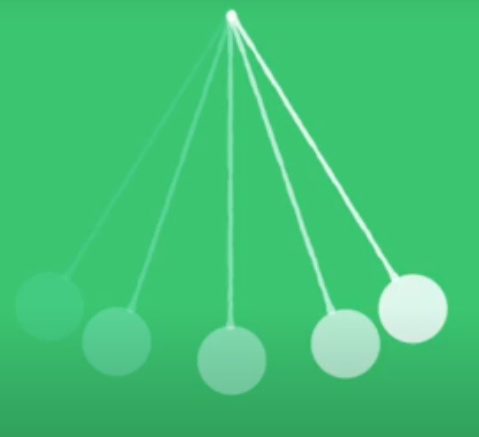
\includegraphics[width=0.3\linewidth]{img/pendolo.png} 
    \caption{Un pendolo oscillante.}
    \label{fig:pendolo}
\end{figure}  


Se si cronometrano le oscillazioni, si vede che, ripetendo la misura, non si ottiene lo stesso tempo. La ragione è che questo tipo di misura è soggetto ad incertezze casuali (ad esempio dovute al tempo di reazione di chi misura, tempo che cambia ogni volta che si ripete la misura stessa). Per ovviare a questo problema, è stata sviluppata una teoria statistica che consente di valutare il miglior valore e l'errore da associare alla misura nel limite in cui si fanno tante misure con strumenti di alta sensibilità. Senza entrare nel merito, ricordiamo semplicemente che il miglior valore risulta la media dei valori :

\[
\overline{T} = \frac{1}{N} \sum_{i=1}^{N} T_i
\]

\noindent
Questo significa che sommiamo tutti i valori $T_1, T_2, \ldots, T_N$ e poi dividiamo per il numero totale di valori $N$. In altre parole:
\[
\overline{T} = \frac{1}{N} (T_1 + T_2 + \cdots + T_N)
\]
Lo sparpagliamento dei dati  è legato alla cosiddetta deviazione standard:

\[
\sigma = \sqrt{\frac{1}{N-1} \sum_{i=1}^{N} (T_i - \overline{T})^2}
\]

\noindent
Questo significa che per ogni valore $T_i$, calcoliamo la differenza tra $T_i$ e la media $\overline{T}$, la eleviamo al quadrato, sommiamo questi quadrati per tutti i valori da $1$ a $N$, dividiamo per $N-1$, e infine prendiamo la radice quadrata. In altre parole:
\[
\sigma = \sqrt{\frac{1}{N-1} \left[ (T_1 - \overline{T})^2 + (T_2 - \overline{T})^2 + \cdots + (T_N - \overline{T})^2 \right]}
\]
(la divisione per $N-1$ anziché per $N$ è una correzione che rende la stima più attendibile quando i dati sono pochi; è la stessa formula usata dai fogli di calcolo con la funzione \texttt{DEV.ST}).

Si assume invece, come incertezza (o errore assoluto), il rapporto tra la deviazione standard e la radice quadrata del numero di dati:
\[
\sigma_{\overline{T}}=\frac{\sigma}{\sqrt{N}}
\] 
Notiamo che questa quantità, diminuisce all'aumentare dei dati perché cresce il denominatore. Su questo punto, torneremo nell'ultimo capitolo di questi appunti.
Dopo aver calcolato l'incertezza, dobbiamo sempre ricordarci di scriverla con una sola cifra significativa. Vedremo più avanti vari esempi su come farlo. Le formule sono abbastanza complesse ma è semplice applicarle con un foglio di calcolo, dove esistono funzioni apposite per questo tipo di calcoli (\texttt{MEDIA}, \texttt{DEV.ST}). \\

Se non possiamo ripetere la misura molte volte (diciamo almeno 30) allora la statistica (ossia le tre formule scritte prima) non ci fornisce risultati attendibili. In tal caso, si segue una strada diversa. L'errore si calcola come semidispersione massima ed è dato dalla formula:
\[
\Delta X = \frac{X_{max}-X_{min}}{2}
\]
dove $X_{max}$  e$X_{min}$ sono il valore massimo e  il valore minimo dei nostri dati. Se questo valore viene più piccolo della sensibilità comunque, si assume come errore assoluto la sensibilità. Infatti,ricordando l'esempio del pendolo, se usiamo un cronometro con sensibilità di 0,1 s, è impossibile distinguere due valori che abbiano una differenza minore di questa quantità. 

Supponiamo di aver misurato il periodo $T$ di oscillazione di un pendolo 5 volte e di aver calcolato la media e la semidispersione, ottenendo $T=\SI{1,21}{s}$ e $\Delta x = \SI{0,51}{s}$. Anzitutto arrotondiamo l'errore ad \underline{una} cifra significativa, ossia $\Delta x \approx \SI{0,5}{s}$, poi arrotondiamo il periodo alla seconda cifra decimale: $T\approx \SI{1,2}{s}$ e , in fine, scriviamo il risultato corretto:
\[
T=\left(1,2 \pm 0,5 \right)\si{\second}
\]
\section[Stima per difetto e per eccesso]{Stima per difetto e per eccesso: l'area di una figura curva}
Non sempre una grandezza si può leggere direttamente su uno strumento, e non sempre si può ripetere la misura molte volte per farne la media. In parecchi casi, però, riusciamo comunque a \emph{racchiuderla} fra due valori: uno sicuramente più piccolo di quello vero, che chiamiamo \textbf{stima per difetto}, e uno sicuramente più grande, la \textbf{stima per eccesso}. Il valore vero, qualunque sia, si trova fra i due. Possiamo allora assumere come miglior valore il punto di mezzo dell'intervallo e come incertezza la sua semiampiezza, con lo stesso ragionamento della semidispersione massima:
\[  \colorboxed{ocre}{
\overline{x}=\frac{x_{ecc}+x_{dif}}{2} \qquad\qquad \Delta x=\frac{x_{ecc}-x_{dif}}{2}}
\]
Un caso tipico è la misura dell'area di una figura dal contorno curvo e irregolare -- una foglia, una macchia d'olio, la superficie di un lago su una carta -- per la quale non esiste una formula geometrica. Si procede così: si ricopia il contorno della figura su un foglio a quadretti (o su carta millimetrata) e si sceglie come unità di misura l'area di un quadretto. Poi si contano due gruppi di quadretti:
\begin{elenco}
\item i quadretti \emph{completamente interni} al contorno; il loro numero, moltiplicato per l'area di un quadretto, dà la stima \textbf{per difetto} (i quadretti interni non bastano a coprire tutta la figura);
\item i quadretti interni \emph{insieme a} tutti quelli attraversati dal contorno, anche solo per un angolino; questa somma, moltiplicata per l'area di un quadretto, dà la stima \textbf{per eccesso} (ora abbiamo contato anche pezzetti di superficie che stanno fuori dalla figura).
\end{elenco}

\begin{figure}[h!]
\centering
\begin{tikzpicture}[scale=0.6,
  interno/.style={fill=green!30},
  bordo/.style={fill=orange!35}]
  \foreach \c in {%
    (2,3),(2,4),(2,5),(3,2),(3,3),(3,4),(3,5),(3,6),(4,2),(4,3),(4,4),(4,5),(4,6),
    (4,7),(5,1),(5,2),(5,3),(5,4),(5,5),(5,6),(5,7),(6,2),(6,3),(6,4),(6,5),(6,6),
    (6,7),(7,2),(7,3),(7,4),(7,5),(7,6),(7,7),(8,2),(8,3),(8,4),(8,5),(8,6),(8,7),
    (9,4),(9,5),(9,6)}
    {\fill[interno] \c rectangle ++(1,1);}
  \foreach \c in {%
    (1,2),(1,3),(1,4),(1,5),(1,6),(2,1),(2,2),(2,6),(2,7),(3,1),(3,7),(3,8),(4,0),
    (4,1),(4,8),(5,0),(5,8),(6,0),(6,1),(6,8),(7,1),(7,8),(8,1),(8,8),(9,1),(9,2),
    (9,3),(9,7),(9,8),(10,3),(10,4),(10,5),(10,6),(10,7)}
    {\fill[bordo] \c rectangle ++(1,1);}
  \draw[gray!45,very thin] (0,0) grid (12,10);
  \draw[ocre,line width=1.3pt] plot coordinates {(2.600,1.600) (2.822,1.482)
    (3.075,1.370) (3.354,1.266) (3.654,1.171) (3.969,1.088) (4.294,1.017)
    (4.625,0.961) (4.957,0.922) (5.283,0.901) (5.600,0.900) (5.918,0.918)
    (6.250,0.952) (6.589,1.002) (6.933,1.068) (7.275,1.150) (7.611,1.248)
    (7.937,1.362) (8.246,1.492) (8.536,1.638) (8.800,1.800) (9.047,1.983)
    (9.286,2.191) (9.515,2.420) (9.731,2.666) (9.931,2.925) (10.113,3.194)
    (10.273,3.470) (10.410,3.749) (10.519,4.027) (10.600,4.300) (10.653,4.580)
    (10.682,4.877) (10.688,5.185) (10.671,5.498) (10.631,5.812) (10.569,6.122)
    (10.484,6.420) (10.378,6.703) (10.249,6.965) (10.100,7.200) (9.921,7.416)
    (9.709,7.622) (9.467,7.816) (9.202,7.997) (8.919,8.163) (8.622,8.311)
    (8.316,8.441) (8.007,8.550) (7.700,8.637) (7.400,8.700) (7.097,8.739)
    (6.781,8.755) (6.455,8.751) (6.122,8.726) (5.788,8.681) (5.454,8.618)
    (5.124,8.538) (4.803,8.441) (4.494,8.328) (4.200,8.200) (3.911,8.051)
    (3.618,7.877) (3.326,7.681) (3.039,7.466) (2.763,7.237) (2.501,6.998)
    (2.259,6.750) (2.042,6.499) (1.854,6.248) (1.700,6.000) (1.581,5.746)
    (1.492,5.476) (1.430,5.195) (1.392,4.908) (1.375,4.619) (1.376,4.332)
    (1.392,4.052) (1.420,3.784) (1.457,3.532) (1.500,3.300) (1.549,3.085)
    (1.606,2.880) (1.675,2.685) (1.755,2.500) (1.850,2.325) (1.961,2.160)
    (2.089,2.005) (2.238,1.860) (2.407,1.725)} -- cycle;
  \draw[|<->|,thick] (0,-0.7) -- (1,-0.7)
    node[right,font=\footnotesize] {\ \SI{1}{cm}};
  \fill[interno] (0,-2.05) rectangle ++(0.8,0.8);
  \node[right,font=\footnotesize] at (0.9,-1.65) {quadretto interno};
  \fill[bordo] (6,-2.05) rectangle ++(0.8,0.8);
  \node[right,font=\footnotesize] at (6.9,-1.65) {quadretto di bordo};
\end{tikzpicture}
\caption{Il contorno di una foglia ricopiato su un foglio a quadretti di lato \SI{1}{cm}. In verde i quadretti tutti interni (stima per difetto), in arancione quelli attraversati dal bordo: i verdi più gli arancioni danno la stima per eccesso.}
\label{fig:area-quadretti}
\end{figure}

\begin{testexample}[\thetcbcounter \, Area di una foglia]
Nella figura \ref{fig:area-quadretti} ogni quadretto ha lato \SI{1}{cm} e vale quindi \SI{1}{cm^2}. Contiamo i quadretti verdi, interamente dentro il contorno: sono $42$. I quadretti arancioni, toccati dal bordo, sono $34$.

La stima per difetto usa i soli quadretti interni:
\[
A_{dif}=42\cdot\SI{1}{cm^2}=\SI{42}{cm^2}
\]
La stima per eccesso aggiunge quelli di bordo:
\[
A_{ecc}=(42+34)\cdot\SI{1}{cm^2}=\SI{76}{cm^2}
\]
L'area vera sta fra questi due valori. Prendiamo come miglior valore la loro media e come incertezza la semidifferenza:
\[
\overline{A}=\frac{76+42}{2}\,\si{cm^2}=\SI{59}{cm^2}
\qquad
\Delta A=\frac{76-42}{2}\,\si{cm^2}=\SI{17}{cm^2}
\]
Arrotondiamo l'errore a una sola cifra significativa, $\Delta A\approx\SI{20}{cm^2}$, e il valore alla stessa posizione, $\overline{A}\approx\SI{60}{cm^2}$:
\[
A=\left(60\pm20\right)\si{cm^2}
\]
L'incertezza relativa vale $E_r=17/59\approx0,29$, cioè circa il $29\,\%$: una misura piuttosto grossolana, come è lecito aspettarsi da una griglia larga rispetto alla figura.
\end{testexample}

\begin{remark}
La precisione di questo metodo dipende da quanto è fitta la griglia. L'incertezza nasce solo dai quadretti di bordo: dimezzando il lato del quadretto, ognuno di essi viene sostituito da quattro quadretti quattro volte più piccoli, ma soltanto quelli ancora attraversati dal contorno restano ``incerti''. Il risultato è che, raffinando la griglia, la stima per difetto e quella per eccesso si avvicinano e $\Delta A$ diminuisce. È lo stesso motivo per cui uno strumento più sensibile fornisce una misura più precisa.
\end{remark}
\section{Incertezza relativa e percentuale}
Data una misura $x=\left( \overline{x} \pm \Delta x \right)$ si definisce incertezza relativa il rapporto:
\[  \colorboxed{ocre}{
E_r =\frac{\Delta x}{\overline{x}}}
\]
L'incertezza relativa è un numero senza unità di misura, generalmente piccolo. Infatti, in un esperimento ben progettato, gli errori sono piccoli, rispetto alla grandezza, e dunque il rapporto è minore di uno. Strettamente legata all'incertezza, c'è l'incertezza percentuale, definita come il prodotto della prima per cento. L'incertezza relativa, consente di confrontare due misure, anche di grandezze diverse. Date due grandezze misurate, \textbf{quella più precisa ha l'incertezza relativa minore}. A titolo di esempio, calcoliamo l'incertezza relativa e percentuale della misura di periodo fatta sopra:
\[
Er=\frac{0,5}{1,2}=0,417
\]
mentre l'errore percentuale vale:
\[
E_{\%} = E_r \cdot 100 = 41,7\, \%
\]
Volendo confrontare la precisione di questa misura con questa misura di massa:
\[
m=\left(0,10 \pm 0,01 \right) \si{g}
\]
devo calcolare l'errore relativo della massa:
\[
E_r = \frac{0,01}{0,10}= 0,1
\]
quindi questa misura è più precisa.
\section{Esercizi}
\begin{esercizio}
E' stato misurato il volume di un oggetto ottenendo il risultato
\[
V=\left( 90,0 \pm 0,4\right)\si{mL}.
\]
Determina il risultato corretto nel sistema SI.\\
\risp{$V=\left( 90,0 \pm 0,4\right)\times10^{-6}\,\si{m^3}$}
\end{esercizio}

\begin{esercizio}
In laboratorio è stata misurata la durata del periodo di un pendolo ottenendo il valore $T=\SI{1,874}{s}$ con una semidispersione di $\Delta T =\SI{0,0291}{s}$. Scrivi il risultato in maniera corretta e calcola l'errore percentuale.\\
\risp{$T=\left(1,87 \pm 0,03\right)\si{s}\text{;} E_{\%}=1,6\%$}
\end{esercizio}

\begin{esercizio}
Un gruppo di studenti ha misurato il periodo di oscillazione di un pendolo semplice per 20 volte. I dati raccolti sono riportati nella tabella \ref{tab:pend}. Calcola la media delle misure del periodo (\(\overline{T}\)) e l'incertezza $\Delta T$ e scrivi il risultato in forma corretta.
\risp{$T=\left(2,16 \pm 0,02\right)\,\si{s}$}
\begin{table}[h!]
\centering
\caption{Misure del periodo di oscillazione di un pendolo}
\label{tab:pend}
\begin{tabular}{cc}
\toprule
\textbf{Numero di occorrenze} & \textbf{Misura del periodo (s)} \\
\midrule
5  & 2,14 \\
4  & 2,15 \\
5  & 2,16 \\
3  & 2,17 \\
3  & 2,18 \\
\bottomrule
\end{tabular}
\end{table}


\end{esercizio}


\begin{esercizio}
E' stato misurato l'intervallo d'incertezza per la massa di un oggetto e si è ottenuto l'intervallo compreso tra $\SI{459,7}{g}$ e $\SI{460,3}{g}$. Determina la massa e il suo errore e scrivi il risultato in forma corretta.\\
 \risp{$M=\left(460,0 \pm 0,3\right)\si{g}$}
\end{esercizio}


\begin{esercizio}
Spiega la differenza tra incertezza assoluta e relativa.
\end{esercizio}

\begin{esercizio}
Elenca le seguenti misure per ordine crescente di precisione.
\begin{multicols}{3}
\begin{elenco}
 \item[a)] $L=\left(20,2 \pm 0,1\right)\si{cm}$
 \item[b)] $M=\left(4,01 \pm 0,01\right)\si{kg}$
 \item[c)] $t=\left(1,22 \pm 0,02\right)\si{s}$ \\
 \risp{b, a, c}
\end{elenco}
\end{multicols}

\end{esercizio}


\section{Confronto tra misure}
Supponiamo che due gruppi di studenti abbiano misurato la densità di un oggetto ottenendo i valori $d_1=\left(6,7 \pm 0,2\right)\si{g/cm^3}$ e $d_2=\left(6,9 \pm 0,2\right)\si{g/cm^3}$. Ci chiediamo: questi due valori sono compatibili? All'apparenza no, perchè sono diversi. Siamo portati a pensare che i materiali siano leggermente diversi, oppure uno dei gruppi abbia sbagliato la presa dati. In realtà, per rispondere correttamente, dobbiamo ricordare che le misure sono incerte e il risultato è un intervallo di valori. Nel primo caso l'intervallo và da un minimo di $\SI{6,5}{g/	cm^3}$ ad un massimo di $\SI{6,9}{g/cm^3}$. Per il secondo gruppo, l'intervallo va da $\SI{6,7}{g/cm^3}$ a $\SI{7,1}{g/cm^3}$. La situazione è rappresentata in figura:

\definecolor{zzttqq}{rgb}{0.6,0.2,0}
\definecolor{uququq}{rgb}{0.25,0.25,0.25}
\definecolor{qqqqzz}{rgb}{0,0,0.6}
\definecolor{zzqqtt}{rgb}{0.6,0,0.2}
\definecolor{qqqqff}{rgb}{0,0,1}
\begin{tikzpicture}[line cap=round,line join=round,>=triangle 45,x=1.0cm,y=1.0cm]
\clip(-0.92,-2.28) rectangle (10.44,3.34);
\fill[pattern color=zzttqq,fill=zzttqq,pattern=north east lines] (2.98,1.02) -- (2.96,0) -- (6,0) -- (6.02,1.02) -- cycle;
\draw [line width=3.6pt,color=zzqqtt] (0,0)-- (6,0);
\draw [line width=3.6pt,color=qqqqzz] (2.98,1.02)-- (8.98,1.02);
\draw (-0.12,-0.14) node[anchor=north west] {$6,5 $};
\draw (6.24,0.4) node[anchor=north west] {$6,9$};
\draw (2.1,1.42) node[anchor=north west] {$6,7$};
\draw (9.1,1.44) node[anchor=north west] {$7,1$};
\draw [line width=2pt,dash pattern=on 2pt off 2pt] (2.96,1.94)-- (2.96,-1.06);
\draw [dash pattern=on 2pt off 2pt] (6.02,1.94)-- (6.02,-1.06);
\draw [color=zzttqq] (2.98,1.02)-- (2.96,0);
\draw [color=zzttqq] (2.96,0)-- (6,0);
\draw [color=zzttqq] (6,0)-- (6.02,1.02);
\draw [color=zzttqq] (6.02,1.02)-- (2.98,1.02);
\begin{scriptsize}
\fill [color=qqqqff] (0,0) circle (1.5pt);
\fill [color=qqqqff] (6,0) circle (1.5pt);
\fill [color=qqqqff] (2.98,1.02) circle (1.5pt);
\fill [color=qqqqff] (8.98,1.02) circle (1.5pt);
\fill [color=uququq] (2.96,0) circle (1.5pt);
\fill [color=uququq] (6.02,1.02) circle (1.5pt);
\end{scriptsize}
\end{tikzpicture}

In questo grafico abbiamo riportato i due intervalli di misura in rosso e blu. La zona tratteggiata indica che i due intervalli hanno una zona in comune, ossia la nostra grandezza potrebbe avere come valore vero un valore compreso tra $6,7$ e $6,9$ ma non sappiamo dire di più. Si dice allora che le due misure sono compatibili. Se i due intervalli non si sovrappongono, allora le misure si dicono incompatibili. Consideriamo ad esempio le misure $d_1 = \left(6,7 \pm 0,1\right)\si{g/cm^3}$ e $d_2 = \left(7,1 \pm 0,1\right)\si{g/cm^3}$: il primo intervallo va da $6,6$ a $6,8$, il secondo da $7,0$ a $7,2$. Nel seguente grafico vediamo che non si sovrappongono.

\begin{tikzpicture}[line cap=round,line join=round,>=triangle 45,x=1.0cm,y=1.0cm]
\clip(-0.92,-2.28) rectangle (14.94,3.34);
\draw [line width=3.6pt,color=zzqqtt] (0,0)-- (5.02,0);
\draw [line width=3.6pt,color=qqqqzz] (7.5,1.02)-- (12.52,1.02);
\draw (-0.32,-0.04) node[anchor=north west] {$6,6 $};
\draw (4.70,-0.04) node[anchor=north west] {$6,8$};
\draw (7.18,1.44) node[anchor=north west] {$7,0$};
\draw (12.20,1.44) node[anchor=north west] {$7,2$};
\begin{scriptsize}
\fill [color=qqqqff] (0,0) circle (1.5pt);
\fill [color=qqqqff] (5.02,0) circle (1.5pt);
\fill [color=qqqqff] (7.5,1.02) circle (1.5pt);
\fill [color=qqqqff] (12.52,1.02) circle (1.5pt);
\end{scriptsize}
\end{tikzpicture}
Come si vede il valore massimo della prima misura, $6,8$, è minore del valore minimo della seconda ($7,0$) dunque non ci sono valori comuni ai due intervalli d'incertezza, per cui le misure sono incompatibili. Questo si può generalizzare al caso di più misure. Se anche un solo intervallo non si sovrappone agli altri, allora le misure sono incompatibili. Ovviamente, se tutte le altre sono vicine tra loro e una sola misura è parecchio diversa, probabilmente gli sperimentatori hanno commesso qualche errore di distrazione in quel momento e la misura andrebbe
 ripetuta o semplicemente ignorata.
 
 \section{Esercizi}
 
\begin{esercizio}
Determina se le seguenti misure sono compatibili ed eventualmente indica quella non compatibile con le altre.
\begin{multicols}{3}
\begin{elenco}
 \item[a)] $\left(20,2 \pm 0,2\right)\si{cm}$\\
 \item[b)] $\left(20,0 \pm 0,1\right)\si{cm}$\\
 \item[c)] $\left(19,0 \pm 0,5\right)\si{cm}$ \\
 \risp{No}
\end{elenco}
\end{multicols}

\end{esercizio} 
 
\begin{esercizio}
Determina se le seguenti misure sono compatibili:
\begin{multicols}{3}
\begin{elenco}
 \item[a)] $\left(210 \pm 5\right)\si{mm}$
 \item[b)] $\left(20,0 \pm 0,6\right)\si{cm}$
 \item[c)] $\left(20.5 \pm 0,1\right)\si{cm}$ \\
 \risp{Si}
\end{elenco}
\end{multicols}

\end{esercizio}   
 
 
 


 
\section{Misure indirette: propagazione degli errori.}\label{sec:propagazione}
Quando si misura una grandezza attraverso un calcolo, l'incertezza presente nei dati si ``propaga'' e la ritroviamo nella misura finale. Il modo con cui le incertezze si propagano viene studiato col metodo della propagazione degli errori. Alla base di questo metodo, ci sono due formule, usate nel caso la formula contenga prodotti/quozienti oppure somme/differenze. Tali formule, è bene dirlo, hanno una bene precisa giusitificazione matematica, ma noi non la forniremo, accontentandoci dei risultati.
\subsection{Somme/differenze}
Supponiamo che 

\[
c=a+b
\]

dove $a$ e $b$ sono grandezze di cui conosciamo l'errore. Quanto valgono il miglior valore di $c$  e il suo errore assoluto $\Delta c$? Ovviamente il miglior valore di $c$ è $\overline{c}=\overline{a}+\overline{b}$ (ad esempio se $a=1$ e $b=3$ allora $c= 4$). Per conoscere invece l'errore assoluto $\Delta c$ dovremmo conoscere l'intervallo di incertezza di $c$, ma $c$ non è stato misurato con uno strumento, ma con un calcolo. Non disponiamo di una riga, una bilancia o qualunque altro strumento per valutare la sensibilità. Dunque non è così ovvio come procedere. I risultati della teoria prevedono che $c$ abbia un valore che è compreso tra $\overline{c} -\Delta c$ e $\overline{c} +\Delta c$ dove l'errore assoluto è semplicemente la somma degli errori:
\[  \colorboxed{ocre}{
\Delta c = \Delta a +\Delta b}
\]

Questa formula quando si applica? Molto semplice. Supponiamo di voler misurare la lunghezza di un tavolo di circa $\SI{1100}{\milli\meter}$ e di disporre di una riga di $\SI{600}{\milli\meter}$ di portata. Allora dovremmo usare \textit{due volte} la riga, una volta per intero   e una volta per una parte in modo che la nostra lunghezza diventi:
\[
\overline{l}= \SI{600}{\milli\meter} +\SI{500}{\milli\meter}=\SI{1100}{\milli\meter}
\]
Dunque, abbiamo fatto un calcolo. Accostando la riga cioè, abbiamo mentalmente fatto una somma perché ci sembra ovvio che, mettendo in fila la riga, le lunghezze si sommino. La teoria ci dice che l'errore sulla lunghezza vale:
\[
\Delta l = \SI{1}{\milli\meter}+\SI{1}{\milli\meter}=\SI{2}{\milli\meter}
\]
in quanto l'errore di lettura sulla riga è di $\SI{1}{\milli\meter}$.

Lo stesso discorso si può fare in altri casi. Supponiamo ad esempio di disporre di una bilancia di portata $\SI{4000}{\gram}$. Se dobbiamo pesare due pacchi di peso $\SI{3500}{\gram}$ e $\SI{2000}{\gram}$, non possiamo metterli entrambi sulla bilancia perchè si romperebbe (lo so l'esempio vi sembra artificioso e vi starete chiedendo ``come fai a sapere quanto pesano senza pesarli?'', ma  si può  valutare  ad occhio la massa.) Poi è sempre meglio essere prudenti in queste cose e se una volta pesati separatamente, vediamo che la somma è minore di $\SI{4000}{\gram}$, allora significa che siamo stati troppo prudenti!). Anche  in questo caso quindi, ricorreremo ad una \underline{somma} e, supponendo che la singola pesata abbia un errore di $\SI{1}{g}$, il nostro risultato è :
\[
M =\left(5500 \pm 2 \right)\si{\gram}
\]
Notiamo che abbiamo preso come errore la somma degli errori, come nel caso precedente.

Questo discorso vale anche per le differenze. La formula analoga alla precedente, nel caso $d=a-b$, è 


\[  \colorboxed{ocre}{
\Delta d = \Delta a + \Delta b}
\]
ossia facciamo \textbf{la somma degli errori}, non la differenza. Un esempio è la misura della'area di una figura cava.
\begin{testexample}[ \thetcbcounter \, Area di un trapezio forato]
 Guardando la figura in basso, si chiede di calcolare l'area della parte in grigio conoscendo l'area esterna e l'area del cerchio. Supponiamo che l'area esterna (trapezio) valga:
\[
A_{tot}=\left (120 \pm 2\right)\si{cm^2}
\]
mentre quella del cerchio
\[
A_{cerc}=\left( 65 \pm 1\right)\si{cm^2}
\]
\definecolor{ffffff}{rgb}{1,1,1}
\begin{tikzpicture}[line cap=round,line join=round,>=triangle 45,x=1.0cm,y=1.0cm]
\clip(-2.86,-0.18) rectangle (10.16,4.14);
\fill[fill=black,fill opacity=0.65] (0,0) -- (4,4) -- (10,4) -- (10,0) -- cycle;
\draw [line width=0.4pt,fill=black,fill opacity=1.0] (6.42,2) circle (1.4cm);
\draw (0,0)-- (4,4);
\draw (4,4)-- (10,4);
\draw (10,4)-- (10,0);
\draw (10,0)-- (0,0);
\draw [color=ffffff](6,2.18) node[anchor=north west] {\textbf{$A_{cerc}$}};
\draw [color=ffffff](2.52,0.92) node[anchor=north west] {\textbf{$A_{est}$}};
\end{tikzpicture}

allora l'area grigia vale:
\[
A_{est}=\left ( 55 \pm  3\right)\si{cm^2}
\]
\end{testexample}
\subsection{Moltiplicazioni/divisioni}
La regola per gli errori sui prodotti è più complessa. Essa afferma che se una grandezza è prodotto o rapporto tra due grandezze, il suo errore relativo si può calcolare direttamente senza calcolare l'errore assoluto. Quindi con i prodotti e quozienti noi calcoliamo subito l'errore relativo. Traduciamo in formule questa frase. Se $c=a \cdot b$, allora:
\[  \colorboxed{ocre}{
\frac{\Delta c}{\overline{c}} =\frac{\Delta a}{\overline{a}}+\frac{\Delta b}{\overline{b}}
}
\]
Questa formula lega l'errore relativo su $c$ a quelli di $a$ e $b$. Facciamo un esempio. Supponiamo di aver misurato i lati $a$ e $b$ di un rettangolo coi relativi errori ottenendo: $a=\left(10,25  \pm 0,05\right)\si{mm}$ e  $b=\left(15,00  \pm 0,05\right)\si{mm}$. L'errore relativo su $c$ è pertanto:
\[
\frac{\Delta c}{\overline{c}}=\frac{0,05}{10,25} +\frac{0,05}{15,00}=0,008211382
\]
Essendo questo un errore relativo, possiamo lasciare qualche cifra significativa in più. Ora calcoliamo l'area :
\[
\overline{A}=\overline{a} \cdot \overline{b} = \SI{10,25}{mm} \cdot \SI{15,00}{mm}  = \SI{153.75}{mm^2} 
\]
Ora ci chiediamo come calcolare l'errore assoluto. Ma sappiamo che l'errore relativo e l'errore assoluto sono legati, e l'errore assoluto, si può calcolare da una formula inversa: $\Delta A = E_r \cdot \overline{A}=0,008211382 \cdot \SI{153.75}{mm^2}=\SI{1,26}{mm^2}	\approx \SI{1}{mm^2}$. In definitiva abbiamo:
\[
A=\left(154 \pm 1\right)\si{mm^2}
\]
Notiamo che abbiamo approssimato l'area per avere lo stesso numero di cifre decimali dell'errore.

\textbf{Osservazione.} In questo esercizio abbiamo calcolato prima l'errore relativo e poi quello assoluto. Se in un problema è richiesto solo l'errore relativo, questo approccio è il più conveniente. In laboratorio di solito, si richiede di calcolare direttamente l'errore assoluto. In tal caso, possiamo verificare che la formula da applicare è:
\[  \colorboxed{ocre}{
\Delta c = \overline{c} \cdot \left(\frac{\Delta a}{\overline{a}} + \frac{\Delta b}{\overline{b}}\right)}
\]
Notiamo che l'unità di misura dell'errore è la stessa di $c$ perché la quantità in parentesi è una somma di errori relativi e quindi non ha unità di misura. Per questo, quando si fanno gli esercizi. è sempre bene effettuare i calcoli portandosi dietro le unità di misura. Notiamo ancora che, in parentesi, c'è una somma di errori relativi. Se uno dei due è molto più piccolo dell'altro, allora possiamo trascurarlo. Questo significa che l'errore relativo finale è l'errore relativo della misura \underline{meno precisa}. Per questo, quando in laboratorio facciamo misure, dobbiamo evitare che una misura rozza ``rovini'' il risultato. Questa formula vale anche se vogliamo calcolare l'errore in un rapporto, ovvero, se $c=\frac{a}{b}$, allora: 

\[
\Delta c = \overline{c} \cdot \left(\frac{\Delta a}{\overline{a}} + \frac{\Delta b}{\overline{b}}\right)
\] 


Facciamo un altro esempio.
\vspace{0.5 cm}
\begin{testexample}[\thetcbcounter \, Densità di un liquido]
Supponiamo di aver misurato la massa e il volume di un liquido ottenendo i risultati: $M=\left(320,0  \pm 0,1 \right)\si{g} $ e $V=\left(407 \pm 1 \right)\si{mL}$. Calcoliamo la densità senza approssimarla:
\[
\overline{d}=\frac{\overline{M}}{\overline{V}}=\frac{\SI{320,0}{g}}{\SI{407}{mL}}=\SI{7,400491}{\frac{g}{mL}}
\]
Ora calcoliamo l'errore:
\[
\Delta d = \overline{d}\cdot \left(\frac{\Delta M}{\overline{M}} +\frac{\Delta V}{\overline{V}}  \right)   = \SI{7,400491}{\frac{g}{mL}}\cdot\left(\frac{0,1}{320,0} +\frac{1}{407}  \right) =\SI{0,02}{\frac{g}{mL}}
\]
In definitiva la nostra densità vale:
\[
d=\left(7,40 \pm 0.02 \right)\si{\frac{g}{mL}}
\]
\end{testexample}


\begin{testexample}[\thetcbcounter \, Velocità media]
Un gruppo di studenti ha misurato il tempo $t=\left(2,3450 \pm 0,0001\right)\,\si{\second}$ impiegato da un carrello, per percorrere  lo spazio percorso $s=\left(1822 \pm 1\right)\,\si{\milli\meter}$.  Determinare la velocità media e il suo errore assoluto e scrivere il risultato in forma corretta nel sistema internazionale: $v = \left( \overline{v} \pm \Delta v\right)\,\si{\meter\per\second}$.


La velocità media $\overline{v}$ si ottiene dividendo lo spazio percorso $s$ per il tempo impiegato $t$:

$$\overline{v} = \frac{\overline{s}}{\overline{t}} = \frac{1822\,\si{\milli\meter}}{2,345\,\si{\second}} = \SI{776,97}{\milli\meter\per\second} =  \SI{0,77697}{\meter\per\second}  $$
Calcolo dell'errore assoluto:
\[
\Delta v = \overline{v}\cdot \left(\frac{\Delta s}{\overline{s}} +\frac{\Delta t}{\overline{t}}  \right) =  \left( \SI{0,77697}{\meter\per\second}\right)\cdot \left(\frac{1}{1822} +\frac{0,0001}{2,3450}  \right) = \SI{0,000459571}{\meter\per\second} \approx \SI{0,0005}{\meter\per\second}.   
\]
In definitiva:
\[
v=\left(0,7770 \pm 0,0005\right) \, \si{\meter\per\second}
\]
Osserviamo che nel calcolo dell'errore relativo, non occorre trasformare i dati nel sistema S.I. perché eventuali fattori di conversione, si semplificherebbero nella frazione. Inoltre, prima di inserire la velocità nella scrittura corretta, l'abbiamo approssimata alla quarta cifra decimale come l'errore. Si noti in fine, che non c'è stato bisogno di riportare i passaggi intermedi per gli errori relativi e applicare le regole sulle cifre significative nella somma, perché, quando si calcolano gli errori, quelle regole non vanno applicate e si può impostare tutto il calcolo direttamente sulla calcolatrice. Stesso discorso quando abbiamo molte potenze di 10: conviene inserirle nella calcolatrice e lasciare che si occupi del calcolo, questo non è un corso di matematica!
 \end{testexample}

\begin{testexample}[\thetcbcounter \, Volume di un parallelepipedo]
Il volume di un parallelepipedo è dato dalla formula:
\[
V=a \cdot b \cdot c
\]
Immaginiamo di avere i seguenti valori dei lati: $a=\left(10,2 \pm 0,1\right)\si{cm}$, $b=\left(8,0 \pm 0,1\right)\si{cm}$, e $c=\left(12,6 \pm 0,1\right)\si{cm}$.
Calcoliamo l'errore assoluto sul volume. La regola del prodotto contiene tre fattori, pertanto avremo:
\[
\Delta V=\overline{V} \cdot \left( \frac{\Delta a}{\overline{a}}+\frac{\Delta b}{\overline{b}} +\frac{\Delta c}{\overline{c}}\right)
\]
Prima calcoliamo il volume: $\overline{V}=\left(\SI{10,2}{cm}\right)\cdot \left(\SI{8,0}{cm}\right)\cdot \left(\SI{12,6}{cm}\right)=\SI{1028,16}{cm^3}$.
L'errore diventa:
\[
\Delta V=\SI{1028,16}{cm^3} \cdot \left( \frac{0,1}{10,2}+\frac{0,1}{8,0} +\frac{0,1}{12,6}\right)=\SI{31,092}{cm^3}
\]
Questo errore ha troppe cifre significative. Per ridurle, possiamo usare la notazione scientifica oppure, un multiplo del centimetro, in modo da ottenere un errore minore di 9 che sappiamo approssimare. Pertanto scriveremo:
\[
\Delta V = \SI{0,031092}{dm^3}\approx \SI{0,03}{dm^3}
\]
Analogamente si ha:
\[
V=\SI{1,02816}{dm^3} 
\]
Dunque la misura finale scritta col corretto numero di cifre significative è:
\[
V=\left(1,03 \pm 0,03\right)\si{dm^3}
\]
Quando gli errori sono maggiori di 10, è concesso lasciare gli zeri ammettendo che, anche se normalmente sarebbero significativi (perché alla fine del numero) in questo caso non lo sono. Quindi, volendo lasciare tutto in centimetri, avremmo anche potuto scrivere:
\[
V=\left(1030 \pm 30\right)\,\si{\cubic\centi\meter}.
\]
\end{testexample}
\begin{testexample}[\thetcbcounter \, perimetro di un quadrato]
Consideriamo un quadrato di lato  $l=\left(10,2 \pm 0,1\right)\si{cm}$. La formula del perimetro è:
\[
\overline{P}=4\overline{l} = 4\cdot \left(\SI{10,2}{\centi\meter} \right) =\SI{40,8}{\centi\meter}.
\]
pertanto, usando la regola per la propagazione dell'errore in un prodotto, abbiamo:
\[
\Delta P= \overline{P}\cdot\left( \cancel{\frac{\Delta 4}{4}} +\frac{\Delta l}{\overline{l}}  \right) = \left(\SI{40,8}{\centi\meter}\right)\cdot \left(\frac{0,1}{10,2} \right) =\SI{0,4}{\centi\meter} .
\]
dove abbiamo cancellato il primo addendo perché 4 (cosi come $\pi$ e tutte le costanti nelle formule) non ha errore (però bisogna metterlo nel calcolo del perimetro). In definitiva abbiamo:
\[
P=\left(40,8 \pm 0,4\right) \si{\centi\meter}.
\]
\end{testexample}




Notiamo che se si ha una formula del tipo:
\[
c=\frac{a\cdot b^2}{d}
\]
ogni fattore al numeratore o al denominatore contribuisce tante volte all'errore relativo quanto è alta la sua potenza perchè la potenza non è altro che una moltiplicazione ripetuta. Dunque, la formula dell'errore diventa:
\[
\Delta c= \overline{c} \cdot \left(\frac{\Delta a}{\overline{a}}+\frac{\Delta b}{\overline{b}} +\frac{\Delta b}{\overline{b}}  +\frac{\Delta d}{\overline{d}} \right)= \left(\frac{\Delta a}{\overline{a}}+2\frac{\Delta b}{\overline{b}}  +\frac{\Delta d}{\overline{d}} \right)
\]
\begin{testexample}[\thetcbcounter \, Misura dell'accelerazione di gravità]
Nella teoria del moto di un oggetto in caduta, si ricava la seguente formula per il calcolo dell'accelerazione di gravità $g$:
\[
g=\frac{2\cdot h}{t^2}
\]
essendo $h$ l'altezza da cui il corpo cade, e $t$ il tempo impiegato a cadere. Vogliamo calcolare l'errore su $g$ supponendo le seguenti misure: $h=\left(6,00 \pm 0,01\right)\si{m}$, e $t=\left(1,11\pm 0,01\right)\si{s}$. Inserendo i valori otteniamo subito: $g = \SI{9,74}{m/s^2}$.
Per l'errore è facile convincersi che la formula da usare è:
\[
\Delta g= \overline{g}\left(\frac{\Delta h}{\overline{h}} +2\frac{\Delta t}{\overline{t}}\right)=\SI{0,19}{m/s^2}\approx \SI{0,2}{m/s^2}
\]
In definitiva:
\[
g=\left(9,7 \pm 0,2\right)\si{m/s^2}
\]
\end{testexample}
\begin{testexample}[\thetcbcounter \,  Volume del cilindro]
Consideriamo un cilindro di raggio $r=\left(1,205 \pm 0,005\right)\si{cm}$ e altezza $h=\left(4,000 \pm 0,005 \right)\si{cm}$. La formula per il calcolo del volume è:
\[
V=\pi\cdot  r^2 \cdot h
\]
pertanto il valore numerico risulta: $V =\SI{18,247}{cm^3}$, mentre per l'errore si ha:
\[
\Delta V=\overline{V}\cdot \left(2\frac{\Delta r}{\overline{r}} +\frac{\Delta h}{\overline{h}}\right)=\SI{0,174}{cm^3}\approx \SI{0,2}{cm^3}
\]
La misura comprensiva dell'errore è pertanto:
\[
V=\left(18,2 \pm 0,2\right)\si{cm^3}
\]
\end{testexample}


\subsection{Esercizi}
\begin{esercizio}
In laboratorio si vuole misurare il volume di un solido irregolare. Per fare questo, si misura inizialmente il volume di una certa quantità d'acqua presente in un becker, ottenendo il valore  $V_i=\left(60 \pm 1\right)\si{mL}$. Una volta inserito il corpo, il livello sale a $V_f=\left(105 \pm 1\right)\si{mL}$. Determina il volume dell'oggetto sommerso e scrivi il risultato in forma corretta.\\
 \risp{$V=\left(45 \pm 2\right)\si{mL}$}
\end{esercizio}

\begin{esercizio}
Si vuole misurare la lunghezza di una stanza utilizzando un metro con portata $\SI{2,000}{m}$ e sensibilità $\SI{0,1}{cm}$. Il valore misurato risulta essere $L=\SI{6,450}{m}$. Scrivi il risultato in forma corretta (hai già il valore della grandezza, ti manca l'errore). Rifletti su come potrebbe essere stata effettuata la misura per capire quanto vale l'errore.\\
 \risp{$L=\left(6,450 \pm 0,003\right)\si{m}$}
\end{esercizio}

\begin{esercizio}
Un pentagono regolare, ha lato $L=\left(2,5 \pm 0,1\right)\si{cm}$. Determina il suo perimetro e scrivi il risultato con l'errore.\\
 \risp{$2P=\left(12,5 \pm 0,5\right)\si{cm}$}
\end{esercizio}
\begin{esercizio}
Viene misurato 10 volte il tempo T di oscillazione di un pendolo, ottenendo i risultati in tabella:

\begin{center}
\begin{tabular}{|c|c|}
\hline 
T(s)& Ripetuto\\
\hline
1,25 & 2 volte\\
1,24 & 4 volte \\
1,23 & 1 volta \\
1,20 & 2 volte \\
1,21 & 1 volta \\
\hline
\end{tabular}
\end{center}
Determina il valore medio e l'errore. In fine, scrivi il risultato in forma corretta.\\
\risp{$T=\left(1,23 \pm 0,03\right)\si{s}$}
\end{esercizio}
\begin{esercizio}
Un modo per misurare l'accelerazione di caduta, è usare la seguente relazione:
\[
g=\frac{v^2}{2 h}
\]
essendo $h$ l'altezza da cui si fa cadere un oggetto, e $v$ la velocità di caduta (misurata con un cronometro fatto partire automaticamente quando l'oggetto cade, tramite una fotocellula). Un gruppo di studenti, ha misurato $h$ e $v$ ottenendo:
\[
h=\left(1226 \pm 1 \right) \, \si{\milli\meter} \text{;}\,\, v=\left(4,8531 \pm  0,0001\right) \, \si{\meter\per\second} 
\]
Determina il valore di $g$ col suo errore e scrivi il risultato in forma corretta. \\\hspace*{\fill} [$g=\left(9,605 \pm 0,008 \right) \, \si{\meter\per\square\second}$] 
\end{esercizio}

\begin{esercizio}
In geometria, il volume di una sfera di raggio $r$ si calcola con la formula:
\[
V=\frac{4\cdot\pi \cdot r^3}{3}
\] 
Supponiamo di aver misurato col calibro il diametro $d$ di una sfera avendo ottenuto $d=\left(9,555 \pm 0,005\right)\si{cm}$. Dimostra che la formula del volume, espressa rispetto al diametro è:
\[
V=\frac{\pi \cdot d^3}{6}
\]
Utilizzando questa formula:
\begin{enumerate}
\item[a)] Calcola il volume;
\item[b)] Scrivi la formula per il calcolo dell'errore;
\item[c)] Calcola l'errore.
\item[d)] Scrivi il risultato in forma corretta.
\end{enumerate}
 \hspace*{\fill}   $\left[\overline{V}=\SI{456.76}{cm^3}\text{,} \Delta V=\overline{V}\cdot\left(3\frac{\Delta d}{d}\right)\approx\SI{0.7}{cm^3}\text{,} V=\left(456,8 \pm 0,7 \right)\si{cm^3}\right] $
\end{esercizio}
\vspace{0.2cm}
\begin{esercizio}
Si sa che una grandezza $f$ dipende dalle grandezze $a$, $b$, $c$, $d$, $e$ attraverso la formula:
\[
f = 4 \cdot \frac{a\cdot b^2 \cdot c^3}{d^4 \cdot e^5}
\]
Determina la formula per il calcolo dell'errore assoluto su $f$.\\

\risp{$\Delta f=\overline{f}\cdot\left(\frac{\Delta a}{\overline{a}}+ 2\cdot \frac{\Delta b}{\overline{b}} +3\cdot\frac{\Delta c}{\overline{c}} + 4\cdot \frac{\Delta d}{\overline{d}} + 5\cdot \frac{\Delta e}{\overline{e}}  \right)$}
\end{esercizio}
\section{Propagazione degli errori indipendenti e casuali}

Nelle misure sperimentali, gli errori casuali associati a grandezze indipendenti si propagano secondo regole specifiche. Questo approccio, basato sulla \textbf{somma in quadratura}, si differenzia dalla propagazione degli errori massimi (strumentali), dove si sommano direttamente i contributi degli errori. Infine, vedremo come combinare un errore casuale con un errore massimo.

\subsection{Somme e differenze}
Per somme o differenze di grandezze indipendenti, l'errore assoluto totale è dato dalla \textbf{somma in quadratura} degli errori assoluti:

\[
\Delta S = \sqrt{(\Delta A)^2 + (\Delta B)^2},
\]
dove $S = A \pm B$.

Questo approccio si applica quando gli errori sono \textbf{casuali e indipendenti}, ed è meno conservativo rispetto alla propagazione degli errori massimi, che semplicemente somma gli errori: $\Delta S = \Delta A + \Delta B$.

\textbf{Esempio.}
Supponiamo di avere $A = 5,0 \pm 0,2$ e $B = 3,0 \pm 0,1$. Calcoliamo $S = A + B$:
\[
S = 5,0 + 3,0 = 8,0,
\]
\[
\Delta S = \sqrt{(0,2)^2 + (0,1)^2} = \sqrt{0,04 + 0,01} = \sqrt{0,05} \approx 0,2.
\]
Risultato: $S = 8,0 \pm 0,2$.  
L'errore assoluto finale è stato arrotondato ad una sola cifra significativa.

\subsection{Prodotti e quozienti}
Per prodotti o quozienti di grandezze indipendenti, gli errori relativi si sommano in quadratura:

\[
\frac{\Delta R}{R} = \sqrt{\left(\frac{\Delta A}{A}\right)^2 + \left(\frac{\Delta B}{B}\right)^2},
\]
dove $R = A \cdot B$ oppure $R = A / B$.  
Da qui, l'errore assoluto risulta:
\[
\Delta R = R \cdot \sqrt{\left(\frac{\Delta A}{A}\right)^2 + \left(\frac{\Delta B}{B}\right)^2}.
\]

\textbf{Esempio.}
Se $A = 5,0 \pm 0,2$ e $B = 3,0 \pm 0,1$, calcoliamo $R = A \cdot B$:
\[
R = 5,0 \cdot 3,0 = 15,0,
\]
\[
\frac{\Delta R}{R} = \sqrt{\left(\frac{0,2}{5,0}\right)^2 + \left(\frac{0,1}{3,0}\right)^2} = \sqrt{0,0016 + 0,0011} \approx 0,053.
\]
\[
\Delta R = 15,0 \cdot 0,053 \approx 0,8.
\]
Risultato: $R = 15,0 \pm 0,8$.

\subsection{Combinazione di errori casuali ed errori massimi}
Se una misura è affetta da un errore casuale $\Delta_c$ e da un errore massimo (strumentale) $\Delta_m$, questi possono essere combinati in quadratura:
\[
\Delta = \sqrt{(\Delta_c)^2 + (\Delta_m)^2}.
\]

\textbf{Esempio.}
Una grandezza $A = 10,0 \pm 0,3$ ha un errore casuale $\Delta_c = 0,3$ e un errore massimo $\Delta_m = 0,5$. L'errore totale sarà:
\[
\Delta A = \sqrt{(0,3)^2 + (0,5)^2} = \sqrt{0,09 + 0,25} = \sqrt{0,34} \approx 0,6.
\]
Risultato: $A = 10,0 \pm 0,6$.

\subsection{Differenze rispetto alla propagazione degli errori massimi}
Con la propagazione degli errori massimi, si assume il caso peggiore, cioè che tutti gli errori si sommino direttamente. Questo approccio è più conservativo ma spesso sovrastima l'incertezza, specialmente se gli errori sono indipendenti e casuali.

Ad esempio, per $A = 5,0 \pm 0,2$ e $B = 3,0 \pm 0,1$, nella propagazione degli errori massimi avremmo:
\[
\Delta S = \Delta A + \Delta B = 0,2 + 0,1 = 0,3,
\]
mentre la somma in quadratura dà $\Delta S \approx 0,2$, che è più realistico.

\subsection{Conclusioni}
La somma in quadratura fornisce un'approssimazione migliore dell'incertezza totale quando gli errori sono casuali e indipendenti, distinguendosi dall'approccio conservativo della propagazione degli errori massimi. La combinazione con errori massimi tramite la somma in quadratura è particolarmente utile per misure sperimentali complesse.
